%==========================================================
% CHAPTER: Funkcijų ribos (A kursas)
%==========================================================
\chapter{Funkcijų ribos (A kursas)}

\section{Ribos sąvoka}

Ribos sąvoka yra viena iš pagrindinių matematinės analizės idėjų. Ji leidžia tiksliai aprašyti, kaip funkcijos reikšmės elgiasi, kai argumentas artėja prie tam tikro taško ar begalybės. Šios sąvokos pagrindu grindžiamos išvestinės, integralai ir daugelis kitų matematikos šakų.

% ─────────────────────────────────────────────
\subsection{Intuityvus ribos supratimas}
% ─────────────────────────────────────────────

\begin{tcolorbox}[colback=blue!5!white, colframe=blue!50!black, title=Pagrindinė idėja]
Sakome, kad funkcijos $f(x)$ \textbf{riba}, kai $x$ artėja prie $a$, lygi $L$, jei funkcijos reikšmės $f(x)$ artėja prie $L$, kai tik $x$ artėja prie $a$ (iš abiejų pusių), nepriklausomai nuo to, ar $f(a)$ apskritai apibrėžta.
\end{tcolorbox}

\subsubsection*{Pavyzdys: artėjimas prie taško}

Nagrinėkime funkciją
\[
    f(x) = \frac{x^2 - 4}{x - 2}.
\]
Šios funkcijos apibrėžimo sritis yra $\mathbb{R} \setminus \{2\}$, nes $x = 2$ vardiklis lygus nuliui. Tačiau galima suprastinti:
\[
    f(x) = \frac{(x-2)(x+2)}{x-2} = x + 2, \quad x \neq 2.
\]
Nors $f(2)$ nėra apibrėžta, stebime, kad kai $x$ artėja prie $2$, $f(x)$ artėja prie $4$:

\begin{center}
\begin{tabular}{c|c}
    $x$ & $f(x) = x + 2$ \\
    \hline
    $1{,}9$ & $3{,}9$ \\
    $1{,}99$ & $3{,}99$ \\
    $1{,}999$ & $3{,}999$ \\
    $2{,}001$ & $4{,}001$ \\
    $2{,}01$ & $4{,}01$ \\
    $2{,}1$ & $4{,}1$ \\
\end{tabular}
\end{center}

Taigi intuityviai rašome:
\[
    \lim_{x \to 2} \frac{x^2 - 4}{x - 2} = 4.
\]

\begin{remark}
Svarbu suprasti: \textbf{riba aprašo elgesį artėjant prie taško, o ne pačiame taške}. Funkcija gali būti neapibrėžta taške $x = a$, tačiau jos riba tame taške vis tiek gali egzistuoti.
\end{remark}

\subsubsection*{Geometrinė interpretacija}

Geometriškai $\lim_{x \to a} f(x) = L$ reiškia, kad funkcijos grafiko taškai artėja prie taško $(a, L)$, kai $x \to a$. Gali būti, kad pačiame $x = a$ grafikas turi „skylutę" (taško trūkumas), tačiau aplinkui grafiko reikšmės artėja prie $L$.

\begin{center}
\begin{tikzpicture}
\begin{axis}[
    axis lines = center,
    xlabel = {$x$},
    ylabel = {$f(x)$},
    xmin = 0, xmax = 4.5,
    ymin = 0, ymax = 6.5,
    xtick = {2},
    xticklabels = {$a$},
    ytick = {4},
    yticklabels = {$L$},
    width = 9cm, height = 7cm,
    grid = both,
    grid style = {line width=0.2pt, draw=gray!30},
]
\addplot[blue, thick, domain=0:1.97, samples=100] {x + 2};
\addplot[blue, thick, domain=2.03:4.5, samples=100] {x + 2};
\addplot[only marks, mark=o, mark size=3pt, blue] coordinates {(2, 4)};
\draw[dashed, gray] (axis cs:2,0) -- (axis cs:2,4);
\draw[dashed, gray] (axis cs:0,4) -- (axis cs:2,4);
\end{axis}
\end{tikzpicture}
\end{center}

\subsubsection*{Vienpusės ribos}

Kartais $x$ artėja prie $a$ tik iš vienos pusės:

\begin{itemize}
    \item \textbf{Kairinioji riba}: $\displaystyle\lim_{x \to a^-} f(x) = L^-$ — $x$ artėja prie $a$ iš kairės (iš mažesnių reikšmių).
    \item \textbf{Dešinioji riba}: $\displaystyle\lim_{x \to a^+} f(x) = L^+$ — $x$ artėja prie $a$ iš dešinės (iš didesnių reikšmių).
\end{itemize}

\begin{theorem}
Dvipusė riba $\displaystyle\lim_{x \to a} f(x) = L$ egzistuoja tada ir tik tada, kai egzistuoja abi vienpusės ribos ir jos lygios:
\[
    \lim_{x \to a^-} f(x) = \lim_{x \to a^+} f(x) = L.
\]
\end{theorem}

\begin{example}
Nagrinėkime modulinę funkciją $f(x) = \dfrac{|x|}{x}$. Tada:
\[
    \lim_{x \to 0^-} \frac{|x|}{x} = \frac{-x}{x} = -1, \qquad
    \lim_{x \to 0^+} \frac{|x|}{x} = \frac{x}{x} = 1.
\]
Kadangi $-1 \neq 1$, dvipusė riba taške $x = 0$ \textbf{neegzistuoja}.
\end{example}

\subsubsection*{Riba begalybėje}

Ribą galima svarstyti ir kai $x \to \pm\infty$:

\begin{itemize}
    \item $\displaystyle\lim_{x \to +\infty} f(x) = L$ reiškia, kad $f(x)$ artėja prie $L$, kai $x$ didėja be apribojimų.
    \item $\displaystyle\lim_{x \to -\infty} f(x) = L$ reiškia, kad $f(x)$ artėja prie $L$, kai $x$ mažėja be apribojimų.
\end{itemize}

\begin{example}
\[
    \lim_{x \to +\infty} \frac{1}{x} = 0, \qquad
    \lim_{x \to -\infty} \frac{1}{x} = 0.
\]
Geometriškai tai reiškia, kad funkcijos $f(x) = \frac{1}{x}$ grafiko horizontalioji asimptota yra $y = 0$.
\end{example}

% ─────────────────────────────────────────────
\subsection{Ribos apibrėžimas}
% ─────────────────────────────────────────────

\subsubsection*{Formalusis apibrėžimas ($\varepsilon$-$\delta$ apibrėžimas)}

Intuityvų „artėjimo" supratimą galima tiksliai suformuluoti naudojant vadinamąjį \textbf{Koši–Veierštaso} ($\varepsilon$-$\delta$) apibrėžimą.

\begin{definition}[Funkcijos riba taške]
Sakome, kad funkcijos $f(x)$ \textbf{riba taške} $a$ yra lygi $L$ ir rašome
\[
    \lim_{x \to a} f(x) = L,
\]
jei kiekvienam $\varepsilon > 0$ egzistuoja toks $\delta > 0$, kad:
\[
    0 < |x - a| < \delta \implies |f(x) - L| < \varepsilon.
\]
\end{definition}

\begin{remark}
Sąlyga $0 < |x - a|$ reiškia, kad $x \neq a$, t.\ y.\ pats taškas $a$ nedalyvauja apibrėžime. Tai patvirtina intuityvią mintį: riba aprašo \emph{artėjimą}, o ne reikšmę $f(a)$.
\end{remark}

\subsubsection*{Apibrėžimo prasmė}

$\varepsilon$-$\delta$ apibrėžimą galima paaiškinti žaidimo metafora:
\begin{enumerate}
    \item \textbf{Oponentas} parenka bet kokį tikslumą $\varepsilon > 0$ (pvz., $\varepsilon = 0{,}001$). Tai yra leistinas nuokrypis nuo $L$.
    \item \textbf{Jūs} turite rasti tokį $\delta > 0$, kad, kai tik $x$ yra $\delta$-aplinkoje aplink $a$ (bet $x \neq a$), funkcijos reikšmė $f(x)$ patektų į $\varepsilon$-aplinką aplink $L$.
    \item Jei \emph{visada} galite rasti tokį $\delta$, riba egzistuoja ir lygi $L$.
\end{enumerate}

\begin{center}
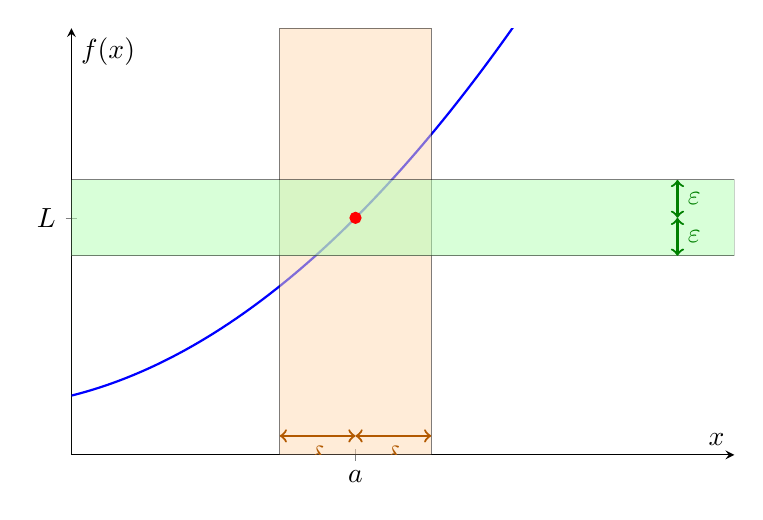
\begin{tikzpicture}
\begin{axis}[
    axis lines = center,
    xlabel = {$x$},
    ylabel = {$f(x)$},
    xmin = 0.5, xmax = 4,
    ymin = 0.5, ymax = 5,
    xtick = {2},
    xticklabels = {$a$},
    ytick = {3},
    yticklabels = {$L$},
    width = 10cm, height = 7cm,
]
% Funkcija
\addplot[blue, thick, domain=0.5:3.95, samples=150] {0.5*x^2 + 1};
% delta juosta
\addplot[fill=orange!30, opacity=0.5] coordinates {(1.6,0.5) (2.4,0.5) (2.4,5) (1.6,5)} \closedcycle;
% epsilon juosta
\addplot[fill=green!30, opacity=0.5] coordinates {(0.5,2.6) (4,2.6) (4,3.4) (0.5,3.4)} \closedcycle;
% Taškai
\addplot[only marks, mark=*, mark size=2pt, red] coordinates {(2, 3)};
% Etiketės
\draw[<->, orange!70!black, thick] (axis cs:1.6, 0.7) -- (axis cs:2, 0.7) node[midway, below] {$\delta$};
\draw[<->, orange!70!black, thick] (axis cs:2, 0.7) -- (axis cs:2.4, 0.7) node[midway, below] {$\delta$};
\draw[<->, green!50!black, thick] (axis cs:3.7, 2.6) -- (axis cs:3.7, 3) node[midway, right] {$\varepsilon$};
\draw[<->, green!50!black, thick] (axis cs:3.7, 3) -- (axis cs:3.7, 3.4) node[midway, right] {$\varepsilon$};
\end{axis}
\end{tikzpicture}
\end{center}

\subsubsection*{Pavyzdys: formalaus apibrėžimo taikymas}

\begin{example}
Įrodykime, kad $\displaystyle\lim_{x \to 3}(2x - 1) = 5$.

\textit{Įrodymas.} Duotas $\varepsilon > 0$. Turime parodyti, kad $|f(x) - 5| < \varepsilon$.

Skaičiuojame:
\[
    |f(x) - 5| = |(2x - 1) - 5| = |2x - 6| = 2|x - 3|.
\]
Norime, kad $2|x - 3| < \varepsilon$, t.\ y.\ $|x - 3| < \dfrac{\varepsilon}{2}$.

Pasirenkame $\delta = \dfrac{\varepsilon}{2}$. Tada, kai $0 < |x - 3| < \delta$:
\[
    |f(x) - 5| = 2|x - 3| < 2\delta = 2 \cdot \frac{\varepsilon}{2} = \varepsilon. \qquad \square
\]
\end{example}

\subsubsection*{Ribų savybės}

Jei $\displaystyle\lim_{x \to a} f(x) = L$ ir $\displaystyle\lim_{x \to a} g(x) = M$, tai galioja šios savybės:

\begin{tcolorbox}[colback=green!5!white, colframe=green!50!black, title=Ribų aritmetika]
\begin{enumerate}
    \item \textbf{Sumos riba:}
    \[
        \lim_{x \to a} [f(x) + g(x)] = L + M.
    \]
    \item \textbf{Skirtumo riba:}
    \[
        \lim_{x \to a} [f(x) - g(x)] = L - M.
    \]
    \item \textbf{Sandaugos riba:}
    \[
        \lim_{x \to a} [f(x) \cdot g(x)] = L \cdot M.
    \]
    \item \textbf{Dalybos riba} (kai $M \neq 0$):
    \[
        \lim_{x \to a} \frac{f(x)}{g(x)} = \frac{L}{M}.
    \]
    \item \textbf{Konstantos sandauga:}
    \[
        \lim_{x \to a} [c \cdot f(x)] = c \cdot L, \quad c \in \mathbb{R}.
    \]
    \item \textbf{Laipsnio riba:}
    \[
        \lim_{x \to a} [f(x)]^n = L^n, \quad n \in \mathbb{N}.
    \]
\end{enumerate}
\end{tcolorbox}

\begin{theorem}[Spaustuvo teorema]
Jei $g(x) \leq f(x) \leq h(x)$ tam tikroje $a$ aplinkoje ir
\[
    \lim_{x \to a} g(x) = \lim_{x \to a} h(x) = L,
\]
tai $\displaystyle\lim_{x \to a} f(x) = L$.
\end{theorem}

\begin{example}
Apskaičiuokime $\displaystyle\lim_{x \to 0} x^2 \sin\!\left(\frac{1}{x}\right)$.

Kadangi $-1 \leq \sin\!\left(\dfrac{1}{x}\right) \leq 1$, tai:
\[
    -x^2 \leq x^2 \sin\!\left(\frac{1}{x}\right) \leq x^2.
\]
Kadangi $\displaystyle\lim_{x \to 0}(-x^2) = 0$ ir $\displaystyle\lim_{x \to 0} x^2 = 0$, pagal spaustuvo teoremą:
\[
    \lim_{x \to 0} x^2 \sin\!\left(\frac{1}{x}\right) = 0.
\]
\end{example}

\subsubsection*{Svarbios ribos}

VBE užduotyse dažnai naudojamos šios standartinės ribos:

\begin{tcolorbox}[colback=yellow!5!white, colframe=yellow!60!black, title=Standartinės ribos]
\begin{align}
    &\lim_{x \to 0} \frac{\sin x}{x} = 1, \\[6pt]
    &\lim_{x \to 0} \frac{1 - \cos x}{x^2} = \frac{1}{2}, \\[6pt]
    &\lim_{x \to \infty} \left(1 + \frac{1}{x}\right)^x = e, \\[6pt]
    &\lim_{x \to 0} \frac{e^x - 1}{x} = 1, \\[6pt]
    &\lim_{x \to 0} \frac{\ln(1+x)}{x} = 1.
\end{align}
\end{tcolorbox}

\subsubsection*{Neapibrėžtumai}

Skaičiuojant ribas dažnai susiduriama su \textbf{neapibrėžtumais} — išraiškomis, kurių tiesioginis skaičiavimas neduoda atsakymo:

\begin{center}
\begin{tabular}{c|l}
    \textbf{Neapibrėžtumo forma} & \textbf{Sprendimo būdas} \\
    \hline
    $\dfrac{0}{0}$ & Suprastinti, išskaidyti dauginamaisiais \\[4pt]
    $\dfrac{\infty}{\infty}$ & Padalyti iš aukščiausio laipsnio \\[4pt]
    $0 \cdot \infty$ & Pertvarkyti į $\frac{0}{0}$ arba $\frac{\infty}{\infty}$ \\[4pt]
    $\infty - \infty$ & Daugyba iš jungtinio \\[4pt]
    $1^\infty,\ 0^0,\ \infty^0$ & Logaritmavimas, rodiklinė forma \\
\end{tabular}
\end{center}

\begin{exercise}
Apskaičiuokite šias ribas:
\begin{enumerate}[label=\alph*)]
    \item $\displaystyle\lim_{x \to 2} \frac{x^2 - 3x + 2}{x - 2}$
    \item $\displaystyle\lim_{x \to \infty} \frac{3x^2 + 5x - 1}{2x^2 - x + 4}$
    \item $\displaystyle\lim_{x \to 0} \frac{\sin(3x)}{x}$
    \item $\displaystyle\lim_{x \to 1} \frac{\sqrt{x} - 1}{x - 1}$
\end{enumerate}
\end{exercise}

\section{Ribų skaičiavimas}

Funkcijos riba yra viena iš pagrindinių matematinės analizės sąvokų. Ji aprašo, kaip funkcija
elgiasi, kai argumentas artėja į tam tikrą reikšmę arba į begalybę. Supratimas apie ribas
yra būtinas norint sėkmingai išmokti išvestines ir integralus.

\begin{definition}
Sakome, kad funkcijos $f(x)$ \textbf{riba}, kai $x$ artėja į $a$, lygi $L$, ir rašome
\[
  \lim_{x \to a} f(x) = L,
\]
jei $f(x)$ reikšmės artėja į $L$, kai $x$ artėja į $a$ iš abiejų pusių (bet $x \neq a$).
\end{definition}

\begin{remark}
Riba gali egzistuoti net tada, kai funkcija taške $x = a$ yra neapibrėžta, t.~y. 
riba apibūdina funkcijos elgesį \emph{aplinkoje} taško, o ne pačiame taške.
\end{remark}

% -------------------------------------------------------
\subsection{Ribų savybės}
% -------------------------------------------------------

Tarkime, kad egzistuoja ribos
\[
  \lim_{x \to a} f(x) = L \quad \text{ir} \quad \lim_{x \to a} g(x) = M,
\]
kur $L, M \in \mathbb{R}$. Tada galioja šios pagrindinės savybės:

\begin{theorem}[Ribų aritmetinės savybės]
\leavevmode
\begin{enumerate}[label=\arabic*.]
  \item \textbf{Sumos (skirtumo) riba:}
  \[
    \lim_{x \to a} \bigl[f(x) \pm g(x)\bigr] = L \pm M.
  \]

  \item \textbf{Sandaugos riba:}
  \[
    \lim_{x \to a} \bigl[f(x) \cdot g(x)\bigr] = L \cdot M.
  \]

  \item \textbf{Konstantos ir funkcijos sandaugos riba:}
  \[
    \lim_{x \to a} \bigl[c \cdot f(x)\bigr] = c \cdot L, \quad c \in \mathbb{R}.
  \]

  \item \textbf{Dalinės ribos:}
  \[
    \lim_{x \to a} \frac{f(x)}{g(x)} = \frac{L}{M}, \quad \text{jei } M \neq 0.
  \]

  \item \textbf{Laipsnio riba:}
  \[
    \lim_{x \to a} \bigl[f(x)\bigr]^n = L^n, \quad n \in \mathbb{N}.
  \]

  \item \textbf{Šaknies riba:}
  \[
    \lim_{x \to a} \sqrt[n]{f(x)} = \sqrt[n]{L}, \quad \text{jei } L \geq 0 \text{ (lyginiam } n\text{)}.
  \]
\end{enumerate}
\end{theorem}

\begin{remark}
Konstantos riba visada lygi tai konstantai:
\[
  \lim_{x \to a} c = c.
\]
Taip pat $\lim_{x \to a} x = a$.
\end{remark}

\begin{example}
Apskaičiuokite $\lim_{x \to 3}(2x^2 - 5x + 1)$.

\textbf{Sprendimas.} Polinomų atveju ribą galima skaičiuoti tiesiog įstatant $x = a$:
\[
  \lim_{x \to 3}(2x^2 - 5x + 1) = 2 \cdot 3^2 - 5 \cdot 3 + 1 = 18 - 15 + 1 = 4.
\]
\end{example}

\begin{theorem}[Sandvičio teorema]
Jei $g(x) \leq f(x) \leq h(x)$ aplinkoje taško $a$ ir
\[
  \lim_{x \to a} g(x) = \lim_{x \to a} h(x) = L,
\]
tai ir $\lim_{x \to a} f(x) = L$.
\end{theorem}

\begin{theorem}[Vienpusės ribos]
Riba $\lim_{x \to a} f(x) = L$ egzistuoja tada ir tik tada, kai egzistuoja abi vienpusės ribos
ir jos lygios:
\[
  \lim_{x \to a^-} f(x) = \lim_{x \to a^+} f(x) = L.
\]
Čia $\lim_{x \to a^-}$ žymi kairę ribą (artėjama iš kairės), o $\lim_{x \to a^+}$ -- dešinę
ribą (artėjama iš dešinės).
\end{theorem}

\begin{example}
Tiriant funkcijos $f(x) = |x|/x$ ribą taške $x = 0$:
\[
  \lim_{x \to 0^+} \frac{|x|}{x} = 1, \qquad \lim_{x \to 0^-} \frac{|x|}{x} = -1.
\]
Kadangi vienpusės ribos skirtingos, riba $\lim_{x \to 0} \frac{|x|}{x}$ \textbf{neegzistuoja}.
\end{example}

\textbf{Ribos begalybėje.} Kai $x \to \pm\infty$, galioja šios pagrindinės formulės:
\[
  \lim_{x \to \infty} \frac{1}{x} = 0, \qquad
  \lim_{x \to \infty} \frac{1}{x^n} = 0 \quad (n > 0), \qquad
  \lim_{x \to \infty} c = c.
\]

% -------------------------------------------------------
\subsection{Algebrinių funkcijų ribos}
% -------------------------------------------------------

Algebrinės funkcijos -- tai polinomai, trupmeninės-racionalios ir iracionalios funkcijos.
Daugeliu atvejų jų ribos skaičiuojamos tiesiogiai įstačius argumento reikšmę.

\begin{theorem}[Tolydžių funkcijų riba]
Jei funkcija $f(x)$ yra tolydi taške $x = a$, tai
\[
  \lim_{x \to a} f(x) = f(a).
\]
\end{theorem}

\textbf{Polinomai.} Kiekvienas polinomas $P(x) = a_n x^n + a_{n-1}x^{n-1} + \cdots + a_0$
yra tolydus visur, todėl:
\[
  \lim_{x \to a} P(x) = P(a).
\]

\begin{example}
\[
  \lim_{x \to -2}(x^3 + 4x - 7) = (-2)^3 + 4(-2) - 7 = -8 - 8 - 7 = -23.
\]
\end{example}

\textbf{Racionalios funkcijos.} Jei $R(x) = P(x)/Q(x)$, tai kiekviename taške, kur
$Q(a) \neq 0$:
\[
  \lim_{x \to a} R(x) = \frac{P(a)}{Q(a)}.
\]

\begin{example}
\[
  \lim_{x \to 1} \frac{x^2 + 2x - 3}{x^2 + x - 2}.
\]
Tiesiogiai įstačius: skaitiklis $1 + 2 - 3 = 0$, vardiklis $1 + 1 - 2 = 0$.
Gauname $\left(\frac{0}{0}\right)$ neapibrėžtumą -- žr.\ sekantį poskyrį.
\end{example}

\textbf{Ribos, kai $x \to \infty$, racionaliosioms funkcijoms.}
Tarkime, $R(x) = \dfrac{a_n x^n + \cdots + a_0}{b_m x^m + \cdots + b_0}$.
Skaitiklį ir vardiklį padalijus iš $x^{\max(n,m)}$, gauname:
\[
  \lim_{x \to \infty} R(x) =
  \begin{cases}
    \dfrac{a_n}{b_n}, & \text{jei } n = m \text{ (laipsniai lygūs)},\\[8pt]
    0,               & \text{jei } n < m \text{ (vardiklis dominuoja)},\\[4pt]
    \pm\infty,       & \text{jei } n > m \text{ (skaitiklis dominuoja)}.
  \end{cases}
\]

\begin{example}
\[
  \lim_{x \to \infty} \frac{3x^2 - x + 5}{2x^2 + 7} = \frac{3}{2}.
\]
Skaitiklyje ir vardiklyje didžiausias laipsnis yra $x^2$, todėl riba lygi aukščiausių
laipsnių koeficientų santykiui.
\end{example}

\begin{example}
\[
  \lim_{x \to \infty} \frac{4x^3 - 1}{x^4 + 2x} = 0,
\]
nes vardiklio laipsnis ($4$) yra didesnis už skaitiklio laipsnį ($3$).
\end{example}

\textbf{Iracionalios funkcijos.} Su šaknimis susiduriame, kai skaičiuojame ribas,
kuriose figūruoja $\sqrt{f(x)}$. Jei argumento reikšmėje nėra neapibrėžtumo, tiesiog
įstatome:
\[
  \lim_{x \to 4} \sqrt{x + 5} = \sqrt{4 + 5} = \sqrt{9} = 3.
\]
Kai neapibrėžtumas atsiranda, dažnai naudojama \textbf{konjugatų technika} (padauginimas
iš jungtinės išraiškos), žr.\ sekantį poskyrį.

% -------------------------------------------------------
\subsection{Neapibrėžtumai \texorpdfstring{$\frac{0}{0}$}{0/0}
            ir \texorpdfstring{$\frac{\infty}{\infty}$}{infty/infty}}
% -------------------------------------------------------

Kai skaičiuodami ribą tiesiogiai įstatę argumento reikšmę gauname $\frac{0}{0}$ arba
$\frac{\infty}{\infty}$, tai vadinama \textbf{neapibrėžtumu}. Tokie rezultatai nereiškia,
kad ribos nėra -- reikia atlikti papildomus algebrinius pertvarkymus.

\begin{tcolorbox}[colback=yellow!10, colframe=orange!80!black, title=Svarbiausia taisyklė]
Neapibrėžtumas $\frac{0}{0}$ ar $\frac{\infty}{\infty}$ \textbf{nereiškia}, kad riba lygi
$0$, $1$, ar kad jos nėra. Tai tik signalas, jog reikia pertvarkyti išraišką.
\end{tcolorbox}

\subsubsection*{Neapibrėžtumas $\dfrac{0}{0}$}

Šis neapibrėžtumas atsiranda, kai $x \to a$ ir tiek skaitiklis, tiek vardiklis artėja į $0$.
Pagrindiniai pašalinimo būdai:

\paragraph{1 būdas: dauginamaisiais skaidymas (faktorizacija).}
Skaitiklį ir vardiklį išskaidome dauginamaisiais ir sutrumpiname bendrą dauginamąjį
$(x - a)$.

\begin{example}
\[
  \lim_{x \to 2} \frac{x^2 - 4}{x^2 - x - 2}
  = \left(\frac{0}{0}\right)
  = \lim_{x \to 2} \frac{(x-2)(x+2)}{(x-2)(x+1)}
  = \lim_{x \to 2} \frac{x+2}{x+1}
  = \frac{4}{3}.
\]
\end{example}

\begin{example}
\[
  \lim_{x \to -1} \frac{x^3 + 1}{x + 1}
  = \left(\frac{0}{0}\right)
  = \lim_{x \to -1} \frac{(x+1)(x^2 - x + 1)}{x+1}
  = \lim_{x \to -1}(x^2 - x + 1)
  = 1 + 1 + 1 = 3.
\]
Čia panaudojome kubo sumą: $x^3 + 1 = (x+1)(x^2 - x + 1)$.
\end{example}

\paragraph{2 būdas: konjugatų technika (su šaknimis).}
Jei neapibrėžtumas susijęs su šaknimis, skaitiklį arba vardiklį padauginame iš
``konjugato'' -- išraiškos, kuri skiriasi tik ženklu prieš šaknį.

\begin{example}
\[
  \lim_{x \to 0} \frac{\sqrt{x+1} - 1}{x}
  = \left(\frac{0}{0}\right).
\]
Padauginame skaitiklį ir vardiklį iš $(\sqrt{x+1} + 1)$:
\[
  = \lim_{x \to 0} \frac{(\sqrt{x+1} - 1)(\sqrt{x+1} + 1)}{x(\sqrt{x+1} + 1)}
  = \lim_{x \to 0} \frac{(x+1) - 1}{x(\sqrt{x+1} + 1)}
  = \lim_{x \to 0} \frac{x}{x(\sqrt{x+1} + 1)}
  = \lim_{x \to 0} \frac{1}{\sqrt{x+1} + 1}
  = \frac{1}{2}.
\]
\end{example}

\begin{example}
\[
  \lim_{x \to 4} \frac{\sqrt{x} - 2}{x - 4}
  = \left(\frac{0}{0}\right)
  = \lim_{x \to 4} \frac{(\sqrt{x} - 2)(\sqrt{x} + 2)}{(x-4)(\sqrt{x}+2)}
  = \lim_{x \to 4} \frac{x - 4}{(x-4)(\sqrt{x}+2)}
  = \lim_{x \to 4} \frac{1}{\sqrt{x}+2}
  = \frac{1}{4}.
\]
\end{example}

\paragraph{Naudingi polinomų skaidymai.}
\begin{align*}
  x^2 - a^2 &= (x-a)(x+a), \\
  x^3 - a^3 &= (x-a)(x^2+ax+a^2), \\
  x^3 + a^3 &= (x+a)(x^2-ax+a^2), \\
  x^n - a^n &= (x-a)(x^{n-1} + x^{n-2}a + \cdots + a^{n-1}).
\end{align*}

\subsubsection*{Neapibrėžtumas $\dfrac{\infty}{\infty}$}

Šis neapibrėžtumas atsiranda, kai $x \to \infty$ ir tiek skaitiklis, tiek vardiklis artėja
į begalybę. Pagrindinis metodas -- \textbf{padalijimas iš aukščiausio laipsnio} $x^k$.

\textbf{Algoritmas:}
\begin{enumerate}[label=\arabic*.]
  \item Nustatome aukščiausią $x$ laipsnį skaitiklyje ($n$) ir vardiklyje ($m$).
  \item Skaitiklį ir vardiklį dalijame iš $x^{\max(n,m)}$.
  \item Naudojame faktą: $\lim_{x\to\infty} \frac{1}{x^k} = 0$ visiems $k > 0$.
\end{enumerate}

\begin{example}
\[
  \lim_{x \to \infty} \frac{5x^3 - 2x + 1}{3x^3 + x^2 - 4}
  = \left(\frac{\infty}{\infty}\right).
\]
Dalijame iš $x^3$:
\[
  = \lim_{x \to \infty}
    \frac{5 - \dfrac{2}{x^2} + \dfrac{1}{x^3}}{3 + \dfrac{1}{x} - \dfrac{4}{x^3}}
  = \frac{5 - 0 + 0}{3 + 0 - 0}
  = \frac{5}{3}.
\]
\end{example}

\begin{example}
\[
  \lim_{x \to \infty} \frac{2x^2 - 3}{4x^3 + x}
  = \left(\frac{\infty}{\infty}\right).
\]
Dalijame iš $x^3$:
\[
  = \lim_{x \to \infty}
    \frac{\dfrac{2}{x} - \dfrac{3}{x^3}}{4 + \dfrac{1}{x^2}}
  = \frac{0 - 0}{4 + 0}
  = 0.
\]
Tai atitinka bendrą taisyklę: kai vardiklio laipsnis didesnis, riba lygi $0$.
\end{example}

\begin{example}
\[
  \lim_{x \to \infty} \frac{x^2 + 5x}{3x - 1}
  = \left(\frac{\infty}{\infty}\right).
\]
Dalijame iš $x^2$:
\[
  = \lim_{x \to \infty}
    \frac{1 + \dfrac{5}{x}}{\dfrac{3}{x} - \dfrac{1}{x^2}}
  = \frac{1 + 0}{0 - 0}.
\]
Vardiklis artėja į $0^+$, skaitiklis -- į $1$, todėl riba lygi $+\infty$.
\end{example}

\textbf{Neapibrėžtumas $\frac{\infty}{\infty}$ su šaknimis.}
Kai figūruoja šaknys, laipsnį nustatome pagal didžiausią laipsnį po šaknimi.
Pavyzdžiui, $\sqrt{x^2 + 1}$ elgiasi kaip $x$ (kai $x \to +\infty$), nes
$\sqrt{x^2+1} \sim x$.

\begin{example}
\[
  \lim_{x \to +\infty} \frac{\sqrt{4x^2 + 1} - x}{x + 3}
  = \left(\frac{\infty}{\infty}\right).
\]
Dalijame skaitiklį ir vardiklį iš $x$ (kai $x > 0$, $\sqrt{x^2} = x$):
\[
  = \lim_{x \to +\infty}
    \frac{\sqrt{4 + \dfrac{1}{x^2}} - 1}{1 + \dfrac{3}{x}}
  = \frac{\sqrt{4} - 1}{1 + 0}
  = \frac{2 - 1}{1}
  = 1.
\]
\end{example}

\subsubsection*{Apibendrinanti lentelė}

\begin{center}
\begin{tabular}{|c|c|c|l|}
  \hline
  \textbf{Neapibrėžtumas} & \textbf{Atsiranda kai} & \textbf{Metodas} & \textbf{Pavyzdys} \\
  \hline
  $\dfrac{0}{0}$ & $x \to a$, $f(a)=g(a)=0$ & Faktorizacija & $\dfrac{x^2-4}{x-2} \to 4$ \\[6pt]
  $\dfrac{0}{0}$ & $x \to a$, šaknys & Konjugatas & $\dfrac{\sqrt{x}-2}{x-4} \to \frac{1}{4}$ \\[6pt]
  $\dfrac{\infty}{\infty}$ & $x \to \infty$ & Dalyba iš $x^k$ & $\dfrac{3x^2}{x^2+1} \to 3$ \\[6pt]
  \hline
\end{tabular}
\end{center}

\begin{exercise}
Apskaičiuokite šias ribas:
\begin{enumerate}[label=\alph*)]
  \item $\displaystyle\lim_{x \to 3} \frac{x^2 - 9}{x - 3}$
  \item $\displaystyle\lim_{x \to 1} \frac{x^3 - 1}{x^2 - 1}$
  \item $\displaystyle\lim_{x \to 9} \frac{\sqrt{x} - 3}{x - 9}$
  \item $\displaystyle\lim_{x \to \infty} \frac{6x^4 - x^2 + 2}{2x^4 + 5x - 1}$
  \item $\displaystyle\lim_{x \to \infty} \frac{x^3 - 2x}{5x^2 + 3}$
  \item $\displaystyle\lim_{x \to \infty} \frac{\sqrt{9x^2 + x} - 3x}{1}$
\end{enumerate}

\textbf{Atsakymai:} a)~$6$;\quad b)~$\dfrac{3}{2}$;\quad c)~$\dfrac{1}{6}$;\quad
d)~$3$;\quad e)~$+\infty$;\quad f)~$\dfrac{1}{6}$.
\end{exercise}

\section{Pirmasis ir antrasis puikūs ribos}

Puikiosios ribos (dar vadinamos „nuostabiosiomis ribomis") yra dvi itin svarbios ribų formulės, kurios dažnai naudojamos sudėtingesnių ribų skaičiavimui. Jos yra pagrindinis 12 klasės matematikos VBE II dalies instrumentas.

% -------------------------------------------------------
\subsection{Pirmasis puikus ribos: \texorpdfstring{$\lim_{x \to 0} \frac{\sin x}{x} = 1$}{lim(sin(x)/x) = 1, kai x->0}}

\begin{tcolorbox}[colback=blue!5!white, colframe=blue!60!black, title=Pirmoji puikioji riba]
\[
  \lim_{x \to 0} \frac{\sin x}{x} = 1
\]
\end{tcolorbox}

\subsubsection*{Geometrinis įrodymas (Sandučio teorema)}

Nagrinėkime vienetinį apskritimą (spindulys $r = 1$) ir kampą $x \in \left(0, \frac{\pi}{2}\right)$.

Palyginkime trijų geometrinių figūrų plotus:
\begin{itemize}
  \item Trikampio $OAB$ plotas: $S_1 = \dfrac{1}{2}\sin x$
  \item Sektoriaus $OAB$ plotas: $S_2 = \dfrac{x}{2}$
  \item Trikampio $OAT$ plotas (kur $T$ – tangentinė taškas): $S_3 = \dfrac{1}{2}\tg x$
\end{itemize}

Kadangi $S_1 \leq S_2 \leq S_3$, gauname:
\[
  \frac{1}{2}\sin x \;\leq\; \frac{x}{2} \;\leq\; \frac{1}{2}\tg x
\]

Dalijame visą nelygybę iš $\dfrac{1}{2}\sin x > 0$:
\[
  1 \;\leq\; \frac{x}{\sin x} \;\leq\; \frac{1}{\cos x}
\]

Paimame atvirkštines reikšmes (keičiame nelygybių kryptis):
\[
  \cos x \;\leq\; \frac{\sin x}{x} \;\leq\; 1
\]

\begin{theorem}[Sandučio (spaustuvo) teorema]
Jeigu $g(x) \leq f(x) \leq h(x)$ aplinkoje taško $a$ ir
\[
  \lim_{x \to a} g(x) = \lim_{x \to a} h(x) = L,
\]
tai $\lim_{x \to a} f(x) = L$.
\end{theorem}

Kadangi $\lim_{x \to 0} \cos x = 1$ ir $\lim_{x \to 0} 1 = 1$, pagal sandučio teoremą:
\[
  \lim_{x \to 0} \frac{\sin x}{x} = 1
\]

Funkcija $f(x) = \dfrac{\sin x}{x}$ yra lyginė, todėl ta pati riba galioja ir kai $x \to 0^-$.

\begin{remark}
Kai $x$ matuojamas laipsniais, formulė pasikeičia:
\[
  \lim_{x \to 0} \frac{\sin x^\circ}{x} = \frac{\pi}{180}
\]
Todėl pirmoji puikioji riba galioja \textbf{tik radianų} sistemoje.
\end{remark}

\subsubsection*{Geometrinė interpretacija}

Kai $x \to 0$, lanko ilgis $x$ ir stygos projekcija $\sin x$ tampa praktiškai lygios. Vadinasi, santykis $\dfrac{\sin x}{x} \to 1$. Tai atspindi faktą, kad mažiems kampams $\sin x \approx x$.

\subsubsection*{Pasekmės ir apibendrinimai}

Iš pirmosios puikiosios ribos išvedamos kitos svarbios ribos:

\begin{corollary}
\[
  \lim_{x \to 0} \frac{\tg x}{x} = 1
\]
\end{corollary}

\begin{proof}
\[
  \lim_{x \to 0} \frac{\tg x}{x}
  = \lim_{x \to 0} \frac{\sin x}{x} \cdot \frac{1}{\cos x}
  = 1 \cdot \frac{1}{1} = 1
\]
\end{proof}

\begin{corollary}
\[
  \lim_{x \to 0} \frac{1 - \cos x}{x^2} = \frac{1}{2}
\]
\end{corollary}

\begin{proof}
Naudojame trigonometrinę tapatybę $1 - \cos x = 2\sin^2\!\dfrac{x}{2}$:
\[
  \lim_{x \to 0} \frac{1 - \cos x}{x^2}
  = \lim_{x \to 0} \frac{2\sin^2\!\frac{x}{2}}{x^2}
  = \lim_{x \to 0} \frac{1}{2} \cdot \left(\frac{\sin\frac{x}{2}}{\frac{x}{2}}\right)^2
  = \frac{1}{2} \cdot 1^2 = \frac{1}{2}
\]
\end{proof}

\begin{corollary}
\[
  \lim_{x \to 0} \frac{\arcsin x}{x} = 1, \qquad
  \lim_{x \to 0} \frac{\arctg x}{x} = 1
\]
\end{corollary}

\subsubsection*{Taikymo pavyzdžiai}

\begin{example}
Apskaičiuokite $\displaystyle\lim_{x \to 0} \frac{\sin 5x}{x}$.

\textbf{Sprendimas.} Padauginame ir padalijame iš $5$:
\[
  \lim_{x \to 0} \frac{\sin 5x}{x}
  = \lim_{x \to 0} 5 \cdot \frac{\sin 5x}{5x}
  = 5 \cdot \lim_{u \to 0} \frac{\sin u}{u}
  = 5 \cdot 1 = 5
\]
kur $u = 5x$.
\end{example}

\begin{example}
Apskaičiuokite $\displaystyle\lim_{x \to 0} \frac{\sin 3x}{\sin 7x}$.

\textbf{Sprendimas.}
\[
  \lim_{x \to 0} \frac{\sin 3x}{\sin 7x}
  = \lim_{x \to 0} \frac{\dfrac{\sin 3x}{3x} \cdot 3x}{\dfrac{\sin 7x}{7x} \cdot 7x}
  = \frac{3}{7} \cdot \frac{\lim_{x\to 0}\dfrac{\sin 3x}{3x}}{\lim_{x\to 0}\dfrac{\sin 7x}{7x}}
  = \frac{3}{7} \cdot \frac{1}{1} = \frac{3}{7}
\]
\end{example}

\begin{example}
Apskaičiuokite $\displaystyle\lim_{x \to 0} \frac{1 - \cos x}{x \sin x}$.

\textbf{Sprendimas.}
\[
  \lim_{x \to 0} \frac{1 - \cos x}{x \sin x}
  = \lim_{x \to 0} \frac{1 - \cos x}{x^2} \cdot \frac{x}{\sin x}
  = \frac{1}{2} \cdot 1 = \frac{1}{2}
\]
\end{example}

% -------------------------------------------------------
\subsection{Antrasis puikus ribos: \texorpdfstring{$\lim_{x \to \infty}\left(1+\frac{1}{x}\right)^x = e$}{lim(1+1/x)^x = e, kai x->inf}}

\begin{tcolorbox}[colback=green!5!white, colframe=green!60!black, title=Antroji puikioji riba]
\[
  \lim_{x \to \infty} \left(1 + \frac{1}{x}\right)^x = e \approx 2{,}718\,281\,828\ldots
\]
\end{tcolorbox}

\subsubsection*{Skaičiaus $e$ reikšmė}

Skaičius $e$ yra natūrinio logaritmo pagrindas – viena iš svarbiausių matematikos konstantų. Jis yra transcendentinis skaičius (nei racionalus, nei algebrinis).

\begin{center}
\begin{tabular}{|c|c|}
\hline
$x$ & $\left(1 + \dfrac{1}{x}\right)^x$ \\
\hline
$1$      & $2{,}000\,000$ \\
$10$     & $2{,}593\,742$ \\
$100$    & $2{,}704\,814$ \\
$1000$   & $2{,}716\,924$ \\
$10000$  & $2{,}718\,146$ \\
$\infty$ & $2{,}718\,281\ldots = e$ \\
\hline
\end{tabular}
\end{center}

\subsubsection*{Įrodymas naudojant logaritmą}

Tegu $y = \left(1 + \dfrac{1}{x}\right)^x$. Imame natūrinį logaritmą:
\[
  \ln y = x \ln\!\left(1 + \frac{1}{x}\right)
\]

Tegul $t = \dfrac{1}{x}$. Kai $x \to \infty$, $t \to 0^+$:
\[
  \lim_{x \to \infty} x \ln\!\left(1 + \frac{1}{x}\right)
  = \lim_{t \to 0^+} \frac{\ln(1 + t)}{t}
\]

Taikome L'Hôpital taisyklę (arba pirmąją puikiąją ribą logaritmams):
\[
  \lim_{t \to 0^+} \frac{\ln(1 + t)}{t}
  = \lim_{t \to 0^+} \frac{\dfrac{1}{1+t}}{1}
  = \frac{1}{1} = 1
\]

Taigi $\ln y \to 1$, vadinasi $y \to e^1 = e$. \qed

\subsubsection*{Kitos ekvivalenčios formos}

Keičiant kintamąjį $t = \dfrac{1}{x}$, gauname:

\begin{tcolorbox}[colback=yellow!5!white, colframe=orange!70!black, title=Lygiavertė forma]
\[
  \lim_{t \to 0} (1 + t)^{1/t} = e
\]
\end{tcolorbox}

Taip pat galioja apibendrinimas:
\[
  \lim_{x \to \infty} \left(1 + \frac{k}{x}\right)^x = e^k, \quad k \in \mathbb{R}
\]

\begin{proof}
\[
  \left(1 + \frac{k}{x}\right)^x
  = \left[\left(1 + \frac{1}{x/k}\right)^{x/k}\right]^k
  \xrightarrow{x \to \infty} e^k
\]
\end{proof}

\subsubsection*{Taikymo pavyzdžiai}

\begin{example}
Apskaičiuokite $\displaystyle\lim_{x \to \infty} \left(1 + \frac{3}{x}\right)^x$.

\textbf{Sprendimas.} Naudojame apibendrintą formulę su $k = 3$:
\[
  \lim_{x \to \infty} \left(1 + \frac{3}{x}\right)^x = e^3
\]
\end{example}

\begin{example}
Apskaičiuokite $\displaystyle\lim_{x \to \infty} \left(\frac{x+2}{x-1}\right)^x$.

\textbf{Sprendimas.} Pertvarkyti trupmeną:
\[
  \frac{x+2}{x-1} = 1 + \frac{3}{x-1}
\]

Tegul $u = x - 1$, tada $x = u + 1$ ir kai $x \to \infty$, $u \to \infty$:
\[
  \lim_{x \to \infty} \left(1 + \frac{3}{x-1}\right)^x
  = \lim_{u \to \infty} \left(1 + \frac{3}{u}\right)^{u+1}
  = \lim_{u \to \infty} \left(1 + \frac{3}{u}\right)^{u} \cdot \lim_{u \to \infty}\left(1 + \frac{3}{u}\right)
  = e^3 \cdot 1 = e^3
\]
\end{example}

\begin{example}
Apskaičiuokite $\displaystyle\lim_{x \to 0} (1 + 2x)^{1/x}$.

\textbf{Sprendimas.} Naudojame ekvivalenčią formą su $t = 2x$:
\[
  (1 + 2x)^{1/x} = \left[(1 + 2x)^{1/(2x)}\right]^2
  \;\xrightarrow{x \to 0}\; e^2
\]
\end{example}

\subsubsection*{Ryšys su eksponentine funkcija}

Antroji puikioji riba tiesiogiai susieta su eksponentinės funkcijos apibrėžimu. Kai $n \to \infty$ imant natūraliuosius skaičius:
\[
  e = \lim_{n \to \infty}\left(1 + \frac{1}{n}\right)^n = \sum_{n=0}^{\infty} \frac{1}{n!} = 1 + 1 + \frac{1}{2!} + \frac{1}{3!} + \cdots
\]

Tai leidžia susieti ribą su eilučių teorija ir eksponentinės funkcijos savybėmis.

\begin{remark}
Abiejų puikiųjų ribų žinojimas leidžia spręsti neapibrėžtumo formas:
\[
  \frac{0}{0}, \quad \frac{\infty}{\infty}, \quad 1^\infty
\]
Pirmoji puikioji riba sprendžia $\dfrac{0}{0}$ tipo neapibrėžtumus, antroji – $1^\infty$ tipo.
\end{remark}

\subsubsection*{Apibendrinimas}

\begin{center}
\renewcommand{\arraystretch}{2}
\begin{tabular}{|l|c|c|}
\hline
\textbf{Savybė} & \textbf{I puikioji riba} & \textbf{II puikioji riba} \\
\hline
Formulė & $\displaystyle\lim_{x \to 0}\frac{\sin x}{x} = 1$ & $\displaystyle\lim_{x \to \infty}\!\left(1{+}\frac{1}{x}\right)^x = e$ \\
\hline
Neapibrėžtumas & $\dfrac{0}{0}$ & $1^\infty$ \\
\hline
Įrodymo metodas & Sandučio teorema & Logaritmavimas + L'Hôpital \\
\hline
Apibendrinimas & $\displaystyle\lim_{x \to 0}\frac{\sin kx}{kx} = 1$ & $\displaystyle\lim_{x \to \infty}\!\left(1{+}\frac{k}{x}\right)^x = e^k$ \\
\hline
\end{tabular}
\end{center}

\section{Funkcijos ištisumas}

Funkcijos ištisumas yra viena svarbiausių sąvokų matematinėje analizėje.
Intuityviai tolydi funkcija yra ta, kurios grafikas nubrėžiamas „nekeliant
pieštuko nuo popieriaus" — be jokių šuolių, spragų ar pertrūkių.

% ──────────────────────────────────────────────────────────────────────────
\subsection{Ištisumo apibrėžimas}
% ──────────────────────────────────────────────────────────────────────────

\begin{definition}[Funkcijos ištisumas taške]
Sakome, kad funkcija $f$ yra \textbf{tolydi} taške $x_0$, jei tenkinamos
trys sąlygos:
\begin{enumerate}
  \item Funkcija apibrėžta taške $x_0$, t.\,y.\ egzistuoja $f(x_0)$;
  \item Egzistuoja riba $\displaystyle\lim_{x \to x_0} f(x)$;
  \item Riba lygi funkcijos reikšmei taške:
        \[
            \lim_{x \to x_0} f(x) = f(x_0).
        \]
\end{enumerate}
\end{definition}

\begin{remark}
Trečioji sąlyga apima abi pirmąsias: jei $\lim_{x\to x_0}f(x)=f(x_0)$,
tai ir riba egzistuoja, ir funkcija apibrėžta. Tačiau jas sąmoningai
išskiriame, kad būtų aiškiau, kuri iš sąlygų pažeidžiama trūkio taške.
\end{remark}

Ekvivalentus ištisumas apibrėžimas per argumento prieaugį:

\begin{definition}[Ištisumas per prieaugį]
Funkcija $f$ yra tolydi taške $x_0$, jei
\[
    \lim_{\Delta x \to 0} \Delta y = 0,
    \qquad \text{kur } \Delta y = f(x_0+\Delta x)-f(x_0).
\]
Kitaip tariant, mažam argumento pokyčiui atitinka mažas funkcijos
reikšmės pokytis.
\end{definition}

\begin{definition}[Vienpusiai ribojimai ir vienpusis ištisumas]
\begin{itemize}
  \item Funkcija $f$ yra \textbf{tolydi iš dešinės} taške $x_0$, jei
        \[
            \lim_{x \to x_0^+} f(x) = f(x_0).
        \]
  \item Funkcija $f$ yra \textbf{tolydi iš kairės} taške $x_0$, jei
        \[
            \lim_{x \to x_0^-} f(x) = f(x_0).
        \]
\end{itemize}
Funkcija yra tolydi taške $x_0$ tada ir tik tada, kai ji yra tolydi iš
kairės \textit{ir} iš dešinės tame taške.
\end{definition}

\begin{definition}[Ištisumas intervale ir atkarpose]
\begin{itemize}
  \item Funkcija yra \textbf{tolydi atvirame intervale} $(a,b)$, jei ji
        tolydi kiekviename to intervalo taške.
  \item Funkcija yra \textbf{tolydi uždarame intervale} $[a,b]$, jei ji
        tolydi kiekviename vidiniame taške $(a,b)$, tolydi iš dešinės
        taške $a$ ir tolydi iš kairės taške $b$.
\end{itemize}
\end{definition}

\subsubsection*{Tolydžių funkcijų pavyzdžiai}

\begin{example}
Parodysime, kad $f(x)=x^2$ yra tolydi taške $x_0=3$.
\begin{enumerate}
  \item $f(3)=9$ — apibrėžta.
  \item $\displaystyle\lim_{x\to 3}x^2=9$ — riba egzistuoja.
  \item $\displaystyle\lim_{x\to 3}x^2=9=f(3)$ — riba lygi reikšmei.
\end{enumerate}
Visos trys sąlygos tenkinamos, todėl $f$ tolydi taške $x_0=3$.
\end{example}

\begin{example}
Polonomai, tiesinės, kvadratinės, eksponentinės ir sinuso/kosinuso
funkcijos yra tolydžios savo visoje apibrėžimo srityje.
\begin{itemize}
  \item $f(x)=a_n x^n+\cdots+a_0$ — tolydi visur $(-\infty;+\infty)$.
  \item $f(x)=e^x$, $f(x)=\sin x$, $f(x)=\cos x$ — tolydžios visur.
  \item $f(x)=\ln x$ — tolydi $(0;+\infty)$.
  \item $f(x)=\dfrac{1}{x}$ — tolydi $(-\infty;0)\cup(0;+\infty)$;
        taške $x=0$ neapibrėžta.
\end{itemize}
\end{example}

\subsubsection*{Tolydžių funkcijų algebrinės savybės}

\begin{theorem}
Jei funkcijos $f$ ir $g$ yra tolydžios taške $x_0$, tai tolydžios yra ir:
\[
  f+g,\quad f-g,\quad f\cdot g,\quad \frac{f}{g}\;(g(x_0)\neq 0).
\]
\end{theorem}

\begin{theorem}[Sudėtinės funkcijos ištisumas]
Jei $g$ tolydi taške $x_0$ ir $f$ tolydi taške $g(x_0)$, tai sudėtinė
funkcija $h(x)=f(g(x))$ yra tolydi taške $x_0$.
\end{theorem}

% ──────────────────────────────────────────────────────────────────────────
\subsection{Ištisumo tyrimas}
% ──────────────────────────────────────────────────────────────────────────

Kai reikia nustatyti, ar funkcija tolydi konkrečiame taške, pirmiausia
tikriname, ar nėra pažeista nors viena iš trijų ištisumas sąlygų.
Taškai, kuriuose ištisumas sulaužytas, vadinami \textbf{trūkio taškais}.

\subsubsection*{Trūkio taškų klasifikacija}

\begin{definition}[Pašalinamas trūkio taškas]
Taškas $x_0$ yra \textbf{pašalinamas trūkio taškas}, jei
\[
    \lim_{x\to x_0^-}f(x)=\lim_{x\to x_0^+}f(x)=L,
    \quad \text{tačiau}\quad f(x_0)\neq L
    \;\text{arba}\; f(x_0) \;\text{neapibrėžta.}
\]
Tokiu atveju trūkį galima „pašalinti" papildant arba pakeičiant funkcijos
reikšmę taške $x_0$: $f(x_0):=L$.
\end{definition}

\begin{example}
Tarkime
\[
  f(x)=\frac{x^2-4}{x-2}.
\]
Taške $x_0=2$ funkcija neapibrėžta. Suprastiname:
\[
  f(x)=\frac{(x-2)(x+2)}{x-2}=x+2,\quad x\neq 2.
\]
Todėl $\lim_{x\to 2}f(x)=4$, bet $f(2)$ neegzistuoja. Taškas $x_0=2$ yra
\textit{pašalinamas trūkio taškas}. Papildžius $f(2):=4$, funkcija tampa
tolydi.
\end{example}

\begin{definition}[I rūšies trūkio taškas (šuolis)]
Taškas $x_0$ yra \textbf{I rūšies trūkio taškas}, jei abi vienpusės ribos
egzistuoja ir yra baigtinės, tačiau
\[
    \lim_{x\to x_0^-}f(x)\neq\lim_{x\to x_0^+}f(x).
\]
Skirtumas $\lim_{x\to x_0^+}f(x)-\lim_{x\to x_0^-}f(x)$ vadinamas
\textbf{funkcijos šuoliu} taške $x_0$.
\end{definition}

\begin{example}
Funkcija
\[
  f(x)=
  \begin{cases}
    x+1, & x<3,\\
    x+5, & x\geq 3.
  \end{cases}
\]
Tikriname taške $x_0=3$:
\[
  \lim_{x\to 3^-}f(x)=3+1=4,\qquad
  \lim_{x\to 3^+}f(x)=3+5=8.
\]
Kadangi $4\neq 8$, taškas $x_0=3$ yra \textit{I rūšies trūkio taškas};
funkcijos šuolis lygus $8-4=4$.
\end{example}

\begin{definition}[II rūšies trūkio taškas]
Taškas $x_0$ yra \textbf{II rūšies trūkio taškas}, jei bent viena
vienpusė riba neegzistuoja arba yra begalinė:
\[
    \lim_{x\to x_0^-}f(x)=\pm\infty
    \quad\text{arba}\quad
    \lim_{x\to x_0^+}f(x)=\pm\infty.
\]
\end{definition}

\begin{example}
Funkcija $f(x)=\dfrac{1}{x}$ taške $x_0=0$:
\[
  \lim_{x\to 0^-}\frac{1}{x}=-\infty,\qquad
  \lim_{x\to 0^+}\frac{1}{x}=+\infty.
\]
Taškas $x_0=0$ yra \textit{II rūšies trūkio taškas} (vertikali asimptotė).
\end{example}

\subsubsection*{Ištisumo tyrimo schema}

Tiriant, ar funkcija $f$ tolydi taške $x_0$, rekomenduojama laikytis šios
tvarkos:

\begin{enumerate}
  \item \textbf{Apibrėžimo sritis.} Ar $x_0$ priklauso $f$ apibrėžimo
        sričiai? Jei ne — taškas bent jau yra trūkio taško kandidatas.

  \item \textbf{Vienpusės ribos.} Apskaičiuojame
        \[
          L^- = \lim_{x\to x_0^-}f(x), \qquad
          L^+ = \lim_{x\to x_0^+}f(x).
        \]

  \item \textbf{Ribos egzistavimas.} Jei $L^-\neq L^+$ arba bent viena
        iš jų begalinė — trūkio taškas (I arba II rūšies). Tyrimas
        baigiamas.

  \item \textbf{Reikšmės sutapimas.} Jei $L^-=L^+=L$, tikriname, ar
        $f(x_0)=L$. Jei ne — pašalinamas trūkio taškas. Jei taip —
        funkcija \textbf{tolydi} taške $x_0$.
\end{enumerate}

\begin{example}[Sudėtingesnė kąpsnių funkcija]
Tiriant funkciją
\[
  g(x)=
  \begin{cases}
    \dfrac{\sin x}{x}, & x\neq 0,\\[6pt]
    2,               & x=0.
  \end{cases}
\]
Taške $x_0=0$:
\begin{enumerate}
  \item $g(0)=2$ — apibrėžta.
  \item $\displaystyle\lim_{x\to 0}\frac{\sin x}{x}=1$ (žinoma riba).
  \item $1\neq 2=g(0)$.
\end{enumerate}
Taškas $x_0=0$ yra \textit{pašalinamas trūkio taškas}. Pakeitus $g(0):=1$,
funkcija taptų tolydi.
\end{example}

\begin{example}[Funkcija su šaknimi ir trupmenomis]
Tyrimas: ar $h(x)=\sqrt{x^2-1}$ tolydi taške $x_0=1$?

Apibrėžimo sritis: $x^2-1\geq0 \Rightarrow x\leq-1$ arba $x\geq1$,
taigi $x_0=1$ yra \textbf{apibrėžimo srities krašto taškas}.

\[
  \lim_{x\to 1^+}\sqrt{x^2-1}=\sqrt{0}=0=h(1).
\]
Kairės pusės riba neegzistuoja (taškas nepriklauso apibrėžimo sričiai iš
kairės). Todėl $h$ yra \textit{tolydi iš dešinės} taške $x_0=1$.
\end{example}

\subsubsection*{Svarbios teoremos apie tolydžias funkcijas}

\begin{theorem}[Tarpinės reikšmės teorema (Bolcano–Koši)]
Jei funkcija $f$ tolydi uždarame intervale $[a,b]$ ir $f(a)\neq f(b)$,
tai su bet kokiu skaičiumi $C$, esančiu tarp $f(a)$ ir $f(b)$, egzistuoja
bent vienas taškas $c\in(a,b)$ toks, kad $f(c)=C$.
\end{theorem}

\begin{corollary}
Jei tolydi funkcija kinta ženklą intervale $[a,b]$, t.\,y.\
$f(a)\cdot f(b)<0$, tai egzistuoja bent viena šaknis $c\in(a,b)$:
$f(c)=0$.
\end{corollary}

\begin{remark}
Tarpinės reikšmės teorema dažnai naudojama įrodyti, kad lygtis turi
sprendinį, ir yra šaknų paieškos metodų (pvz., pusiaukirtos metodo)
pagrindas.
\end{remark}

\begin{theorem}[Weierstrasso teorema]
Jei funkcija $f$ tolydi uždarame intervale $[a,b]$, tai ji pasiekia savo
didžiausią reikšmę $M$ ir mažiausią reikšmę $m$ tame intervale:
\[
    \exists\, x_1,x_2\in[a,b]:\quad
    f(x_1)=m=\min_{[a,b]}f,\qquad
    f(x_2)=M=\max_{[a,b]}f.
\]
\end{theorem}

\begin{exercise}
Nustatykite trūkio taško tipą funkcijai
\[
  f(x)=\frac{x^2-9}{x-3}
\]
taške $x_0=3$, o tada papildykite funkciją taip, kad ji taptų tolydi.
\end{exercise}

\begin{exercise}
Raskite konstantą $k$ taip, kad funkcija
\[
  f(x)=
  \begin{cases}
    kx+1, & x\leq 2,\\
    x^2-1,& x>2
  \end{cases}
\]
būtų tolydi taške $x_0=2$.
\end{exercise}

\begin{exercise}
Naudodamiesi tarpinės reikšmės teorema įrodykite, kad lygtis
$x^3-x-1=0$ turi bent vieną sprendinį intervale $(1;\,2)$.
\end{exercise}

